\documentclass{article}

\usepackage[utf8]{inputenc}
\usepackage{graphicx}
\usepackage{caption}
\usepackage{float}
\usepackage{epigraph}
\usepackage{multicol}
\usepackage[bottom,flushmargin]{footmisc} 

\usepackage{adjustbox}
\usepackage{tikz}
\usetikzlibrary{automata, positioning,arrows.meta}
\usetikzlibrary{babel}
\usetikzlibrary{decorations.text}
\usetikzlibrary{decorations.pathreplacing}
\newcommand{\emptystr}{\varepsilon}

\usetikzlibrary{automata, positioning, arrows,
fit, % for the dashed boxes on Thompson's construction
calc
}
\tikzset{%
  node distance=3cm, % specifies the minimum distance between two nodes. Change if necessary.
  every state/.style={thick}, % sets the properties for each ’state’ node
  double distance=2.5pt,
  shorten >= 2pt, shorten <= 2pt,
  initial text=$ $,
  every edge/.style={%
    draw,->, >=stealth, auto, semithick
  }
}

\usepackage{hyperref}
\hypersetup{pdfauthor={Cristian Adrián Ontivero}}
\usetikzlibrary{shapes}
\graphicspath{{imgs/}}

\newlength\tindent
\setlength{\tindent}{\parindent}
\setlength{\parindent}{0pt}
\renewcommand{\indent}{\hspace*{\tindent}}

%These tell TeX which packages to use.
\usepackage{array,epsfig}
\usepackage{amsmath}
\usepackage{amsfonts}
\usepackage{amssymb}
\usepackage{amsxtra}
\usepackage{amsthm}
\usepackage{mathrsfs}

%Here I define some theorem styles and shortcut commands for symbols I use often
\theoremstyle{definition}
\newtheorem{defn}{Definición}
\newtheorem{thm}{Teorema}
\newtheorem{cor}{Corolario}
\newtheorem*{rmk}{Remark}
\newtheorem{lem}{Lema}
\newtheorem*{joke}{Joke}

\newtheorem{ex}{Ejemplo}
\newcommand{\exautorefname}{Ejemplo}

\newtheorem{exercise}{Ejercicio}
\newcommand{\exerciseautorefname}{Ejercicio}

\newtheorem{soln}{Solución}
\newtheorem{prop}{Proposición}

\newcommand{\lra}{\longrightarrow}
\newcommand{\ra}{\rightarrow}
\newcommand{\surj}{\twoheadrightarrow}
\newcommand{\graph}{\mathrm{graph}}
\newcommand{\bb}[1]{\mathbb{#1}}
\newcommand{\Z}{\bb{Z}}
\newcommand{\Q}{\bb{Q}}
\newcommand{\R}{\bb{R}}
\newcommand{\C}{\bb{C}}
\newcommand{\N}{\bb{N}}
\newcommand{\M}{\mathbf{M}}
\newcommand{\m}{\mathbf{m}}
\newcommand{\MM}{\mathscr{M}}
\newcommand{\HH}{\mathscr{H}}
\newcommand{\Om}{\Omega}
\newcommand{\Ho}{\in\HH(\Om)}
\newcommand{\bd}{\partial}
\newcommand{\del}{\partial}
\newcommand{\bardel}{\overline\partial}
\newcommand{\textdf}[1]{\textbf{\textsf{#1}}\index{#1}}
\newcommand{\img}{\mathrm{img}}
\newcommand{\ip}[2]{\left\langle{#1},{#2}\right\rangle}
\newcommand{\inter}[1]{\mathrm{int}{#1}}
\newcommand{\exter}[1]{\mathrm{ext}{#1}}
\newcommand{\cl}[1]{\mathrm{cl}{#1}}
\newcommand{\ds}{\displaystyle}
\newcommand{\vol}{\mathrm{vol}}
\newcommand{\cnt}{\mathrm{ct}}
\newcommand{\osc}{\mathrm{osc}}
\newcommand{\LL}{\mathbf{L}}
\newcommand{\UU}{\mathbf{U}}
\newcommand{\support}{\mathrm{support}}
\newcommand{\AND}{\;\wedge\;}
\newcommand{\OR}{\;\vee\;}
\newcommand{\Oset}{\varnothing}
\newcommand{\st}{\ni}
\newcommand{\wh}{\widehat}

%Pagination stuff.
\setlength{\topmargin}{-.3 in}
\setlength{\oddsidemargin}{0in}
\setlength{\evensidemargin}{0in}
\setlength{\textheight}{9.in}
\setlength{\textwidth}{6.5in}
\pagestyle{empty}

\def\isodate{\leavevmode\hbox{\the\year-\twodigits\month-\twodigits\day}}
\def\twodigits#1{\ifnum#1<10 0\fi\the#1}
\begin{document}
\begin{center}
  {\LARGE Rough Notes on Automata and Formal Languages}\\[.2cm]
  Cristian Adrián Ontivero \\[.05cm]%
  \isodate
\end{center}

\tikzset{reversed/.style={{Latex}-, >=stealth, auto, semithick}}
\begin{figure}[htp]
  \centering
  \begin{tikzpicture}[node distance=5cm, every edge/.style={draw,-{Latex}, >=stealth, auto, semithick}]
    \node[rectangle, draw] at (5,18) (enfa) {$\emptystr$-NFA};
    \node[rectangle, draw, node distance=3cm, right of=enfa] (nfa) {NFA};
    %\node[rectangle, draw, below left of=nfa]  (mnfa) {Minimal NFA};
    \node[rectangle, draw, node distance=8cm, below right of=nfa] (dfa) {DFA};
    \node[rectangle, draw, below of=dfa, node distance=3cm] (mdfa) {Minimal DFA};
    \node[rectangle, draw, node distance=8cm, right of=nfa] (re) {Regular Expression};
    \node[rectangle, draw, below left of=nfa, node distance=3cm] (rlg) {Right-Linear Grammar};
    \node[rectangle, draw, below of=rlg, node distance=2cm] (llg) {Left-Linear Grammar};


    \draw[reversed, postaction={decorate, decoration={text along path, text align=center, raise=4pt, text={McNaughton-Yamada construction}}}] (enfa) to [bend left] (re);
    \draw[reversed, postaction={decorate, decoration={text along path, text
    align=center, raise=4pt, text={Glushkov's construction (Position Automaton)}}}] (nfa) to (re);
    \draw[reversed, postaction={decorate, decoration={text along path, text align=center, raise=4pt, text={Brzozowski's algorithm}}}] (dfa) to [bend left] (re);
    \draw[-{Latex}, >=stealth, auto, semithick, postaction={decorate, decoration={text along path, text align=center, raise=-10pt, text={Brzozowski algebraic method}}}] (dfa) to [bend right] (re);
    \draw[-{Latex}, >=stealth, auto, semithick, postaction={decorate, decoration={text along path, text align=center, raise=4pt, text={Rabin-Scott powerset construction}}}] (nfa) to (dfa);

    \path[bend right=15]
          (rlg) edge node {} (llg)
          (llg) edge node {} (rlg)
          (rlg) edge node {} (nfa)
          (nfa) edge node {} (rlg);
          %(nfa) edge node [above, midway, align=center, minimum width=2.3cm] {Rabin-Scott\\powerset\\construction} (dfa)
          %(dfa) edge node [below, align=center, minimum width=2.3cm]
          %{Brzozowski algebraic method %Transitive closure method, \\ State removal method } (re);
          
          \path
		(enfa) edge node[above] {$\emptystr$-closure} (nfa)
		(dfa) edge node [anchor=center, xshift=1.7cm] {%
            Moore's algorithm%,\\
            %Brzozowski's algorithm,\\
            %Hopcroft's algorithm
	} (mdfa);
            %\path (nfa) edge[densely dotted] node [above, midway] {PSPACE~\cite{MS72}} (mnfa); 
  \end{tikzpicture}
  \caption{\label{fig:lang-automata-equivalences} Some equivalences with their algorithms.}
\end{figure}

Remember that a DFA is (trivially) also an NFA, so any conversion that applies to an NFA applies, too, to a DFA.

The McNaughton-Yamada construction from \cite{MY60} has traditionally been
called Thompson's construction due to a similar construction given by Ken
Thompson. Although neither of the two papers talk about NFAs, that's what they
are using if one reads between the lines.

\iffalse % interesting, but not relevant for the ITBA course.
NFA minimization (the problem of finding a minimal NFA given a certain NFA) is
PSPACE-complete~\cite{MS72}, and the solution is not guaranteed to be unique.
It cannot be efficiently approximated within a factor $O(n)$, unless
$\text{P}=\text{PSPACE}$~\cite{GS07}, and is NP-hard for acyclic unambiguous
finite automata that have a state $q$ with two transitions on the same
symbol~\cite{BM12}.
\fi

Aside from Moore's algorithm for DFA state minimization, there is also Hopcroft's and Brzozowski's.



\newpage

\subsubsection*{McNaughton-Yamada Construction}

\tikzset{fitbox/.style={draw=red, dashed, inner sep=.2cm, rounded corners=.2cm}}
\begin{figure}[ht] % ’ht’ tells LaTeX to place the figure ’here’ or at the top of the page
\centering % centers the figure
\begin{tikzpicture}[node distance=2cm, every state/.style={thick, minimum size=16pt}]
  
    \node[state, initial] (q0) {};
    \node[state, right of=q0, accepting] (q1) {};
    \node[inner sep=.5cm, label=below:empty set: $\varnothing$, fit=(q0) (q1)] (b10) {};

    \node[state, initial, right of=q1, node distance=3cm] (q2) {};
    \node[state, right of=q2, accepting] (q3) {};
    \draw (q2) edge node {$\emptystr$} (q3);
    \node[inner sep=.5cm, label=below:empty string: $\emptystr$, fit=(q2) (q3)] (b11) {};

    \node[state, initial, right of=q3, node distance=3cm] (q4) {};
    \node[state, right of=q4, accepting] (q5) {};
    \draw (q4) edge node {\tt a} (q5);
    \node[inner sep=.5cm, label=below: {\tt \{a\}}, fit=(q4) (q5)] (b12) {};


    \node[state, below of=q2, node distance=3cm] (q7) {};
    \node[state, right of=q7] (q8) {};
    \node[state, below of=q7] (q9) {};
    \node[state, right of=q9] (q10) {};
    \node[fitbox, fit=(q7) (q8)] (b0) {};
    \node[fitbox, fit=(q9) (q10)] (b1) {};
    \node at ($(b0.west)!0.5!(b0.east)$) {\tt R};
    \node at ($(b1.west)!0.5!(b1.east)$) {\tt S};
    \node[inner sep=.5cm, label=below:alternation: {\tt R|S}, fit=(q7) (q8) (q9) (q10)] (b13) {};

    \coordinate (middle-left0) at ($(b0.north west)!0.5!(b0.south west)$);
    \coordinate (middle-left1) at ($(b1.north west)!0.5!(b1.south west)$);
    \coordinate (middle-right0) at ($(b0.north east)!0.5!(b0.south east)$);
    \coordinate (middle-right1) at ($(b1.north east)!0.5!(b1.south east)$);
    \coordinate (between-boxes-left) at ($(middle-left0)!0.5!(middle-left1)$);
    \coordinate (between-boxes-right) at ($(middle-right0)!0.5!(middle-right1)$);

    \node[state, initial, left of=between-boxes-left] (q6) {};
    \node[state, accepting, right of=between-boxes-right] (qn) {};

    \draw (q6) edge node[sloped, anchor=center, above] {$\emptystr$} (q7);
    \draw (q6) edge node[sloped, anchor=center, below] {$\emptystr$} (q9);
    \draw (q8) edge node[sloped, anchor=center, above] {$\emptystr$} (qn);
    \draw (q10) edge node[sloped, anchor=center, below] {$\emptystr$} (qn);

    \node[state, below of=q9, node distance=3cm] (q12) {};
    \node[state, initial, left of=q12] (q11) {};
    \node[state, right of=q12] (q13) {};
    \node[state, accepting, right of=q13] (q14) {};
    \node[fitbox, fit=(q12) (q11)] (b2) {};
    \node[fitbox, fit=(q13) (q14)] (b3) {};
    \coordinate (midpoint1) at ($(b2.north east)!0.5!(b2.south east)$);
    \coordinate (midpoint2) at ($(b3.north west)!0.5!(b3.south west)$);
    \node at ($(b2.west)!0.5!(b2.east)$) {\tt R};
    \node at ($(b3.west)!0.5!(b3.east)$) {\tt S};
    \node[inner sep=.5cm, label=below:concatenation: {\tt RS}, fit=(q11) (q12) (q13) (q14)] (b14) {};

    \draw (q12) edge node {$\emptystr$} (q13);

    \node[state, below of=q12, node distance=3cm] (q15) {};
    \node[state, initial, left of=q15] (q16) {};
    \node[state, right of=q15] (q17) {};
    \node[state, accepting, right of=q17] (q18) {};
    \node[fitbox, fit=(q15) (q17)] (b4) {};
    \node at ($(b4.west)!0.5!(b4.east)$) {\tt R};
    \coordinate (midpoint-left) at ($(b4.north west)!0.5!(b4.south west)$);
    \coordinate (midpoint-right) at ($(b4.north east)!0.5!(b4.south east)$);
    \draw (q16) edge node {$\emptystr$} (midpoint-left);
    \draw (midpoint-right) edge node {$\emptystr$} (q18);
    \draw (q17) edge[bend right=80, looseness=1.5] node[sloped, below]
    {$\emptystr$} (q15);
    \draw (q16) edge[bend right=40] node[above] {$\emptystr$} (q18);
    \node[inner sep=1.4cm, label=below:Kleene closure: $\text{\tt R}^*$, fit=(q15) (q16) (q17) (q18)] (b15) {};

  \end{tikzpicture}
\caption{The McNaughton-Yamada construction, a regular-expression-to-$\emptystr$-NFA construction.}
\label{fig:my_label}
\end{figure}

\subsubsection*{Linear Grammar}
A context free grammar $G = (V, \Sigma, S, P)$ is called a \textbf{linear
grammar} if each of its productions has at most one nonterminal in the right
hand side. That is, each rewriting rule has one of the following two forms:
\begin{align*}
	A &\to \alpha \\
	A &\to \alpha B \beta
\end{align*}
where $A, B \in V$, and $\alpha, \beta \in \Sigma^*$.
Among linear grammars, two special types are right-linear grammars, and
left-linear grammars. The grammar $G$ is said to be right-linear if all
productions are of the form
\begin{itemize}
\item Right-Linear Grammar: these are the grammars that Chomsky defined as type-3 grammars. Their productions have the forms:
\begin{align*}
	A &\to aB\\
	A &\to a
\end{align*}
where $A,B \in V$, and $a \in \Sigma_{\emptystr}$ (i.e. $a$ is either a terminal
symbol, or $\emptystr$).
\item Left-Linear Grammar:
\begin{align*}
	A &\to Ba\\
	A &\to a
\end{align*}
\end{itemize}
Both right-linear grammars and left-linear grammars generate exactly the regular
languages, i.e. they are equivalent to each other.

\iffalse
\begin{enumerate}
\item Take the grammar to right-linear form, i.e. all productions should have
  the form $A \to a$ or $A \to aB$, where $a$ is either a terminal in the
  grammar or $\emptystr$.
\item Label the start state of the NFA with the start symbol of the grammar.
\[
\begin{tikzpicture} \node[state, initial] (S) {$S$}; \end{tikzpicture}\\
\]
\item For each production $A \to aB$, add a state transition (edge) from a state $A$ to a state $B$, and label the edge with the symbol a.
\[
\begin{tikzpicture}
    \node[state] (A) {A};
    \node[state, right of=A] (B) {B};
    \draw (A) edge node {a} (B);
\end{tikzpicture}
\]
\item For each production $A \to B$, add a state transition (edge) from a state
  $A$ to a state $B$, and label the edge with $\emptystr$.
\[
\begin{tikzpicture} 
    \node[state] (A) {A};
    \node[state, right of=A] (B) {B};
    \draw (A) edge node {$\emptystr$} (B);
\end{tikzpicture}
\]
\item If there is any production of the form $A \to a$, add a single new state symbol F. Then for each production of the form $A \to a$, add a state transition from A to F labeled with symbol a. &
\[
\begin{tikzpicture} 
    \node[state] (A) {A};
    \node[state, right of=A] (F) {F};
    \draw (A) edge node {$a$} (B);
\end{tikzpicture}
\]
\item The final states of the NFA are F plus all B such there is a production of
  the form $B \to \emptystr$. &
\[
\begin{tikzpicture}
    \node[state] (A) {A};
    \node[state, accepting, right of=A] (F) {F};
    \node[state, accepting, below of=F, node distance=1.2cm] (B) {B};
    \draw (A) edge node {$a$} (F);
\end{tikzpicture}
\]
\end{enumerate}
\fi

\subsubsection*{Rabin-Scott Powerset Construction}
Rabin and Scott came up with the following construction to prove the equivalence
of NFAs and DFAs~\cite{RS59}. Since a DFA qualifies as an NFA by definition,
proving that an NFA may be converted to a DFA is all that remains.

Given an NFA $A = (Q,\Sigma, \delta,q_0,F)$, we can construct an equivalent DFA $A' = (Q', \Sigma, \delta', q_0', F')$, where:
\begin{itemize}
\item $Q' = \mathcal{P}(Q)$
\item $q_0' = \{q_0\}$
\item $F' = \{S \subseteq Q: S\cap F \neq \emptyset \}$
\item $\delta'(S,a) = \bigcup\limits_{q \in S} \delta(q,a)$
\end{itemize}

As an example, given the NFA from \autoref{fig:nfa-example}, the reader may
corroborate that following the previous construction one reaches the equivalent
DFA shown in \autoref{fig:dfa-example}.

\begin{figure}[htp]
  \centering
\begin{tikzpicture}[node distance=3cm, every state/.style={thick}]  
    \node[state, initial] (q0) {$q_0$};
    \node[state, accepting, right of=q0] (q1) {$q_1$};

    \draw[loop above] (q0) edge node {a,b} ();
    \draw[bend left=10] (q0) edge node {a} (q1);
    \draw[bend left=10] (q1) edge node {b} (q0);
\end{tikzpicture}
\caption{\label{fig:nfa-example} Simple NFA}
\end{figure}

\begin{figure}[htp]
  \centering
\begin{tikzpicture}[node distance=2.5cm, every state/.style={thick, minimum size=38pt}]  
    \node[state, initial] (q0) {\footnotesize $\{q_0\}$};
    \node[state, accepting, below of=q0] (q1) {\footnotesize $\{q_1\}$};
    \node[state, accepting, right of=q0] (q2) {\footnotesize $\{q_0, q_1\}$};
    \node[state, right of=q1] (q3) {\footnotesize $\emptyset$};
    \draw[loop above] (q0) edge node {b} (q2);
    \draw[bend left=10] (q0) edge node {a} (q2);
    \draw[bend left=10] (q2) edge node {b} (q0);
    \draw (q1) edge node {b} (q0);
    \draw (q1) edge node {a} (q3);
\end{tikzpicture}
\caption{\label{fig:dfa-example} Equivalent DFA}
\end{figure}

Unfortunately, since the states of the DFA are, by the previous construction,
$\mathcal{P}(Q)$, an $n$-state NFA leads to a $2^n$ states DFA, even though
sometimes not all of the states are needed (they are \textit{useless}). An
alternative version of the construction tends to produce less states, and is as
follows: 

TODO explicar
\begin{enumerate}
  \item
    \begin{tabular}{r|c|c}
       & $a$ & $b$  \\\hline
       $\{q_0\}$ & $\{q_0, q_1\}$ & $\{q_0\}$
    \end{tabular}
  \item 
    \begin{tabular}{r|c|c}
       & $a$ & $b$  \\
      \hline
       $\{q_0\}$ & $\{q_0, q_1\}$ & $\{q_0\}$ \\
       $\{q_0,q_1\}$ & $\{q_0, q_1\}$ & $\{q_0, q_1\}$
    \end{tabular}
\end{enumerate}

% With the "optimized" powerset construction

\begin{tikzpicture}[node distance=3cm, every state/.style={thick, minimum size=38pt}]  
    \node[state, initial] (q0) {\footnotesize $\{q_0\}$};
    \node[state, accepting, right of=q0] (q1) {\footnotesize $\{q_0, q_1\}$};

    \draw[bend left=10] (q0) edge node {a} (q1);
    \draw[loop above] (q0) edge node {b} (q0);

    \draw[loop above] (q1) edge node {a} (q1);
    \draw[bend left=10] (q1) edge node {b} (q0);
\end{tikzpicture}

Still, there exists languages that require the exponential growth of states when
going from a minimal NFA that recognizes them, to a DFA (even if the DFA is
minimal!). That is, for every $n \in \mathbb{N}$, there is an $n$-state NFA
whose equivalent minimal DFA requires $2^n$ states.

\subsubsection*{Left-Linear Grammar to Right-Linear Grammar}
A left-linear grammar may be converted into a right-linear grammar, simply by
replacing each rule of one of the forms in the first column of , into the
corresponding rule in the second column.
\begin{tabular}{r|l}
  $S \to a$ & $S \to a$ \\
  $A \to a$ & $S \to aA$ \\
  $B \to Aa$ & $A \to aB$ \\
  $S \to Aa$ & $A \to a$
\end{tabular}

\begin{enumerate}
\item If the LLG has a rule $S \to a$, add that rule in to the RLG.
\item If the LLG has a rule $A \to a$, add the rule $S \to aA$ to the RLG.
\item If the LLG has a rule $B \to Aa$, add the rule $A \to aB$ to the RLG.
\item If the LLG has a rule $S \to Aa$, add the rule $A \to a$ to the RLG.
\end{enumerate}

% Taken almost verbatim from Hein's Theory of Computation, p. 312
\tikzset{small-style/.style={double distance=1pt, shorten >= 2pt, shorten <=
  2pt, node distance=1.5cm, every state/.style={thick, inner sep=0pt, minimum
size=16pt}}}
\subsubsection*{Regular Grammar to NFA}

\iftrue % ====================================================================
\newcounter{counter}\stepcounter{counter}
{\setlength{\tabcolsep}{12pt}
\renewcommand{\arraystretch}{2}
\begin{tabular}[t]{@{\hspace{12pt}\arabic{counter}.~\stepcounter{counter}}p{.70\textwidth}p{.25\textwidth}}
Take the grammar to right-linear form, i.e. all productions should have the form
$A \to a$ or $A \to aB$, where $a$ is either a terminal in the grammar or
$\emptystr$. & \\
Label the start state of the NFA with the start symbol of the grammar. &
\adjustbox{valign=t}{\begin{tikzpicture}[small-style]
	\node[state, initial] (S) {$S$};
\end{tikzpicture}}\\
For each production $A \to aB$, add a state transition (edge) from a state $A$ to a state $B$, and label the edge with the symbol $a$. &
\adjustbox{valign=t}{\begin{tikzpicture}[small-style]  
    \node[state] (A) {A};
    \node[state, right of=A] (B) {B};
    \draw (A) edge node {a} (B);
\end{tikzpicture}}\\
For each production $A \to B$, add a state transition (edge) from a state $A$ to
a state $B$, and label the edge with $\emptystr$. &
\adjustbox{valign=t}{\begin{tikzpicture}[small-style]  
    \node[state] (A) {A};
    \node[state, right of=A] (B) {B};
    \draw (A) edge node {$\emptystr$} (B);
\end{tikzpicture}}\\
If there is any production of the form $A \to a$, add a single new state symbol F. Then for each production of the form $A \to a$, add a state transition from A to F labeled with symbol a. &
\adjustbox{valign=t}{\begin{tikzpicture}[small-style]  
    \node[state] (A) {A};
    \node[state, right of=A] (F) {F};
    \draw (A) edge node {$a$} (B);
\end{tikzpicture}}\\
The final states of the NFA are F plus all B such there is a production of the
form $B \to \emptystr$. &
\adjustbox{valign=t}{\begin{tikzpicture}[small-style] 
    \node[state] (A) {A};
    \node[state, accepting, right of=A] (F) {F};
    \node[state, accepting, below of=F, node distance=1cm] (B) {B};
    \draw (A) edge node {$a$} (F);
\end{tikzpicture}}\\
\end{tabular} }
\fi

% Taken almost verbatim from Hein's Theory of Computation, p. 312
\subsubsection*{NFA to Regular Grammar}
The following algorithm produces a regular grammar (specifically, a right-linear grammar) from an NFA:
\begin{enumerate}
\item Rename the states to a set of capital letters.
\item Set the grammar's start symbol to the NFA's start state.
\item For each state transition from A to B labeled with a ($\delta(A,a) = B$), create the production $A \to aB$.
\item For each state transition from A to B labeled with $\emptystr$
  ($\delta(A,\emptystr) = B$), create the production $A \to B$.
\item For each final state F, create the production $F \to \emptystr$.
\end{enumerate}

%\newpage 
\bibliography{refs}
\bibliographystyle{alpha}

\end{document}


